\section{Integración}
\label{sec:integracion}

Para la integración de OpenL Tablets con {\SIDOSPU} existen dos alternativas.

La primera consiste en exponer las reglas por medio de un servicio web utilizando OpenL Rule Services. Esto nos permite integrar con distintas aplicaciones, sobre distintas plataformas, utilizar varias fuentes de datos y exponer varios proyectos y/o módulos mediante un único servicio web.

La segunda alternativa consiste en incluir OpenL Tablets como biblioteca y generar clases wrapper. 
Estas últimas se generan en tiempo de ejecución a partir del contenido de las tablas en documentos Excel, exponiendo las reglas definidas en los mismos como métodos.
La principal ventaja de esta opción es que resulta en un menor costo de comunicación, dado que se realiza por medio de llamadas a métodos entre clases Java.

Considerando que las reglas serán utilizadas únicamente por {\SIDOSPU}, y estarán en un único proyecto, no pudiéndose sacar partido de los beneficios de un servicio web, se decidió utilizar la segunda opción. 
%
%
El diagrama en la \cref{fig:integration} muestra un esquema de la integración resultante. 
Los rectángulos representan una o varias clases Java, siendo la comunicación entre las mismas por llamado de sus respectivos métodos.

\begin{figure*}
    \centering
    \begin{tikzpicture}[
        auto,
        inner sep=3mm,
        box/.style={draw, rectangle, align=center},
        alt-box/.style={draw, rectangle, align=center, rounded corners=12pt},
        pre/.style={Stealth-},
        post/.style={-Stealth},
        alt-pre/.style={dashed, Stealth-},
        alt-post/.style={dashed, -Stealth},
    ]
        \node[box] (system) {SI-DOSPU};
        \node[box, right=of system] (service) {CalculoReglasServiceImpl}
            edge[pre] (system);
        \node[box, below=0.5cm of service] (clases) {Clases Integración}
            (clases.west) edge[post] (system);
        \node[box, right=of service] (wrapper)  {Clase Wrapper}
            edge[pre] (service)
            edge[post] (clases.east);
        \node[alt-box, above=of wrapper] (rules)  {Reglas (excel)}
            edge[alt-post] node {\small Compilado a} (wrapper)
            (rules.west) edge[alt-pre] node[swap] {\small Lee} (service);
    \end{tikzpicture}
    \caption{Integración OpenL Tablets con SI-DOSPU}
    \label{fig:integration}
\end{figure*}


\subsection{Clases de integración}\label{ssec:integracion:clases}

Como se mencionó en el \cref{sec:motores}, OpenL Tablets permite hacer uso directo de objetos Java dentro de las reglas. 
Asimismo, permite hacer uso de clases de forma directa.
Sin embargo, las clases el {\SIDOSPU} lidia con cuestiones no del todo relevantes para el cálculo de las cuotas, como el manejo de errores y el acceso a datos que involucra comunicación con varias clases. Para evitar que estos aspectos se infiltren en las reglas de cálculo, se crearon clase que abstraen estos aspectos, \scode{Afiliacion}, \scode{Valores}. Además, se creó una clase \scode{Numero} para poder operar sobre valores de tipo \scode{BigDecimal} utilizando operadores comunes (+, -, *, /, etc.).



\subsection{Formato de las tablas}

OpenL Tablets ofrece una variedad de tipos de tablas con distintas utilidades, en este trabajo se hizo uso de tablas de configuración, búsqueda y decisión. 
La tabla de decisión posee la mayor flexibilidad y es la utilizada para la mayor parte de la lógica implementada. La presentada más abajo es una versión considerablemente simplificada del formato de las tablas de este tipo, el formato detallado de las tablas, así como sus particularidades pueden encontrarse en la documentación \cite{openl-decision-table}.

\begin{description}
    \item[Fila 1: ] tipo de tabla y signatura.
    \item[Fila 2: ] define si la/s columna/s es/son una condición o retorno.
    \item[Fila 3: ] expresiones (de retorno o condiciones) escritas en \acrshort{bex}.
    \item[Fila 4: ] parámetros utilizados en las expresiones (1 por columna).
    \item[Fila 5: ] nombres descriptivos para los parámetros, ignorados por el motor.
    \item[Fila 6+:] valores concretos para los parámetros. También pueden contener expresiones matemáticas o llamadas a otras reglas.
\end{description}

En el \cref{tbl:calculo:jubilado} se pueden ver las tablas correspondientes al cálculo de la cuota base (sin aportes adicionales) de la subcategoría voluntario jubilado (ver \cref{sssec:jubilado}). Los parámetros de las reglas utilizan las clases de integración mencionadas (ver \cref{ssec:integracion:clases}) Se eligió esta parte de las reglas de negocio dado que es el cálculo más complejo dentro de las subcategorías, ocupando más de 150 líneas de código en la implementación original en el \acrshort{si}.

\begin{table*}
    \centering
    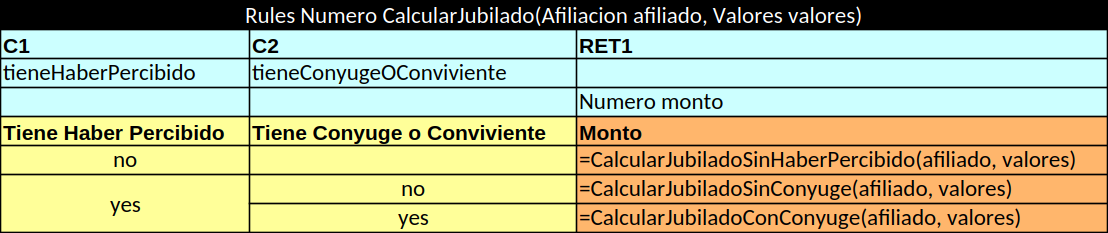
\includegraphics[width=0.9\textwidth]{jubilado.png}
    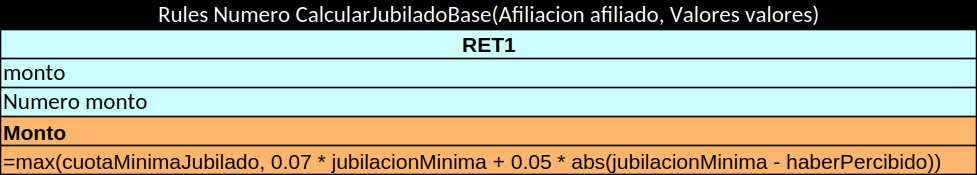
\includegraphics[width=0.8\textwidth]{jubiladoBase.png}
    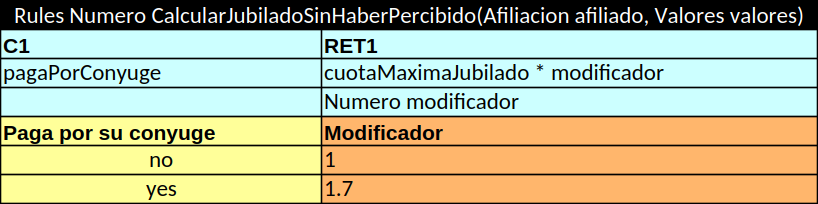
\includegraphics[width=0.65\textwidth]{jubiladoSinHaber.png}
    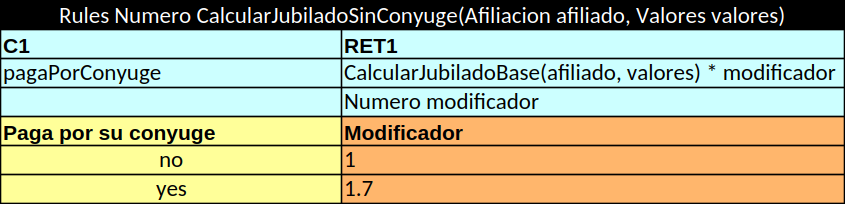
\includegraphics[width=0.7\textwidth]{jubiladoSinConyuge.png}
    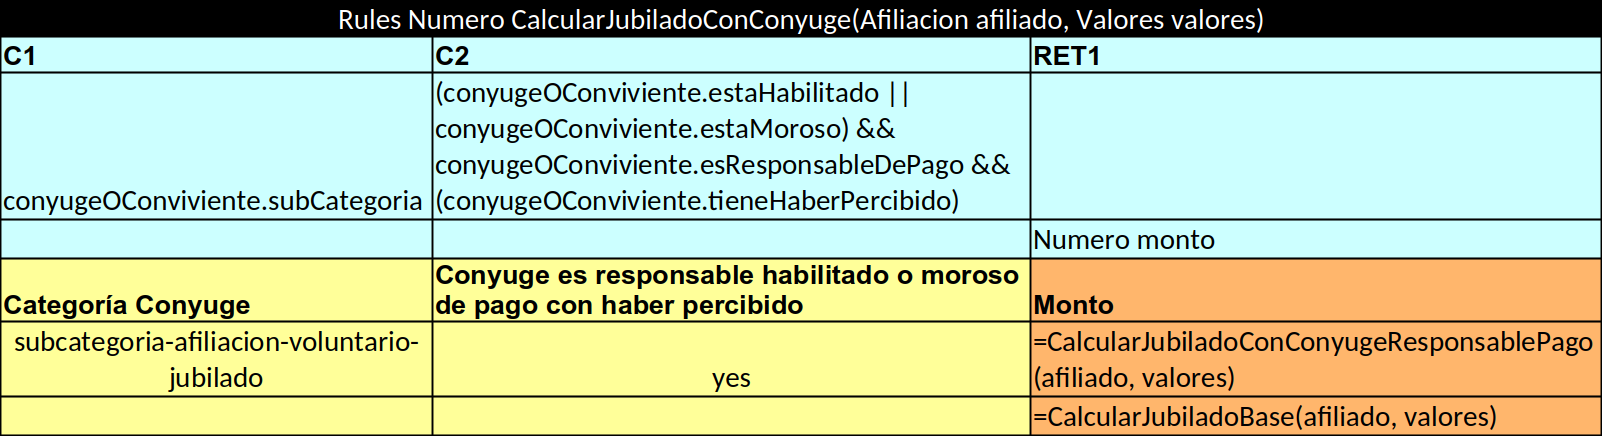
\includegraphics[width=\textwidth]{jubiladoConConyuge.png}
    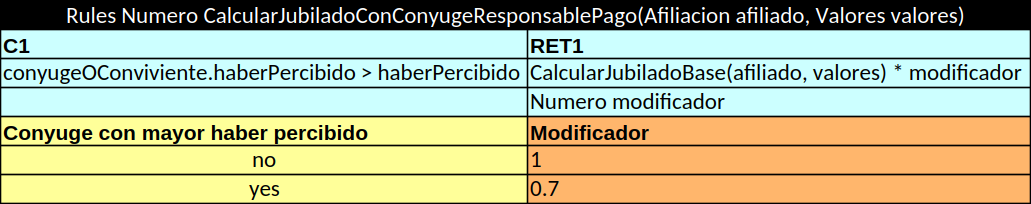
\includegraphics[width=0.8\textwidth]{jubiladoConConyugeResponsable.png}
    \caption{Cálculo cuota base jubilado}
    \label{tbl:calculo:jubilado}
\end{table*}

\subsection{Realizando un cambio}\label{ssec:integracion:cambio}
Para ilustrar las ventajas de estos cambios en el \SIDOSPU a la hora de realizar cambios en las reglas, consideremos la aplicación del siguiente cambio en el valor de las cuotas:

\emph{
Para el cálculo de la cuota de un afiliado con categoría voluntario adherente y subcategoría agente \acrshort{unsl} con licencia, el monto de la cuota es equivalente al monto de los aportes y contribuciones 9\% del sueldo bruto que percibiría como si estuviera en actividad. De igual forma, dicho monto no puede ser inferior a los porcentajes de la \acrshort{cmmu} que se utilizan en el cálculo anteriormente presentado para la categoría y subcategoría.
}

Sin el uso del motor de reglas, este cambio implica el cambio/adición de una 32 líneas de código. Seguidamente, se debe volver a compilar y desplegar el sistema hacer estos cambios efectivos.

Por otra parte, haciendo uso del OpenL Tablets, con la integración descrite, se requiere realizar los cambios entre los cuadros \ref{tbl:cambio:original} y \ref{tbl:cambio:cambiado}. El cambio es detectado en tiempo de ejecución y se generan las nuevas clases wrapper, sin necesidad de volver a compilar o desplegar el sistema.

\begin{table*}
    \centering
    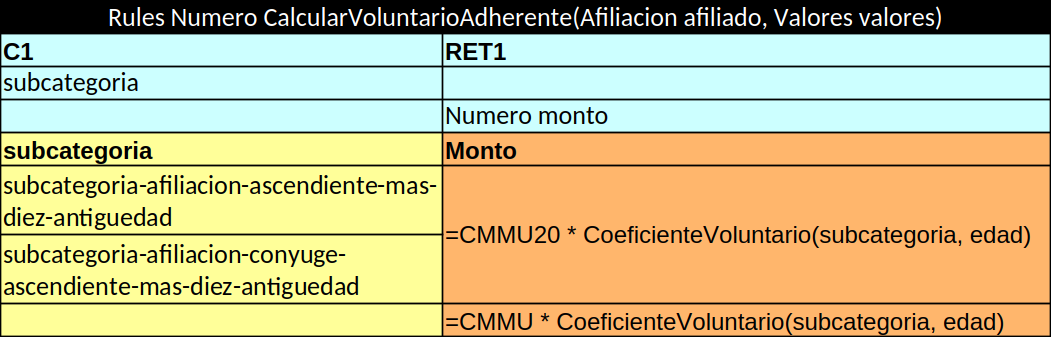
\includegraphics[width=0.8\textwidth]{voluntario.png}
    \caption{Cálculo modificado voluntario adherente}
    \label{tbl:cambio:original}
\end{table*}

\begin{table*}
    \centering
    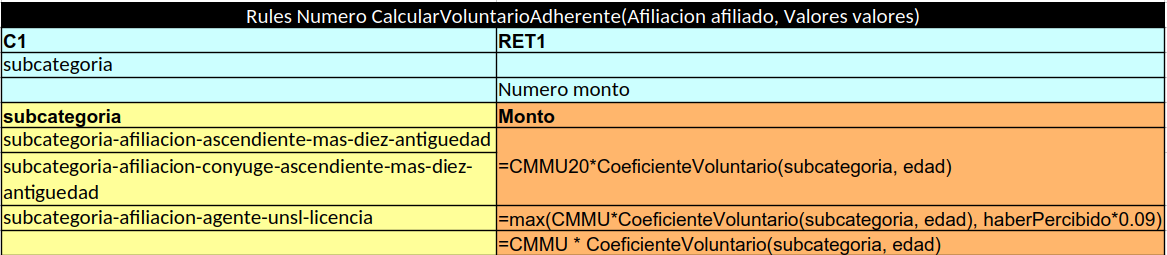
\includegraphics[width=0.8\textwidth]{voluntario_cambios.png}
    \caption{Cálculo modificado voluntario adherente modificado}
    \label{tbl:cambio:cambiado}
\end{table*}
